\documentclass[12pt]{article}
	
\usepackage[margin=1in]{geometry}
\usepackage{graphicx} % Required for inserting images
\usepackage[spanish]{babel}
\usepackage{ragged2e}
\usepackage{atbegshi}  % Required to position graphics
\usepackage[absolute,overlay]{textpos}
\usepackage{titlesec}
\usepackage{titling}
\usepackage{xcolor}
\usepackage{tabularx}
\usepackage{multirow}
\usepackage{enumitem}
\usepackage{booktabs}
\usepackage{graphicx}

\title{Ingeniería Software --- Proyecto semestral \\ Entrega 1 }
\author{\textbf{Grupo 5} \\ Cristobal Fuentealba, Joaquín León, Nicolás Pizarro,\\ Nicolás Soto, Ana María Vargas}
\date{\today}

\setlength{\droptitle}{1cm}

\begin{document}

\begin{textblock*}{5cm}(0.5cm,1cm)
  
\includegraphics[width=2cm]{escudo_udec.png}
\end{textblock*}

\begin{textblock*}{0.8\paperwidth}(0.13\paperwidth,4cm)
  \large{UNIVERSIDAD DE CONCEPCIÓN -- FACULTAD DE INGENIERÍA}
\end{textblock*}

\maketitle

\section{Introducción}

La Organización de Las Naciones Unidas (ONU) buscaba principalmente el crecimiento económico y dejaba de lado el tema del desarrollo humano y medio ambiente. Se ha propuesto la Agenda 2030 para el Desarrollo Sostenible, un ambicioso marco de referencia compuesto por 17 Objetivos de Desarrollo Sostenible (ODS). Esta agenda, ratificada por 193 Estados miembros, es el camino a seguir para un desarrollo socio-económico y ambiental con vistas al año 2030.

Las instituciones de Educación Superior, como la Universidad de Concepción, desempeñan un papel clave en la contribución hacia este esfuerzo global, sin embargo, el monitoreo que sigue las contribuciones de la Universidad a las ODS aún se presenta como un desafío. Aquí radica nuestro problema central de información.

Para resolver este problema, se propone el desarrollo de una solución software que permita a los principales responsables de la universidad monitorear su contribución a los ODS. Este sistema permitirá que los 3  ejes de acción, Formación, Investigación y Vinculación con el Medio, demuestren explícitamente su contribución a los ODS.

Los administradores de la Universidad podrán consultar estos datos, con indicadores claros que reflejen el estado actual de la contribución a los ODS y su progreso en el tiempo. Del mismo modo, también ayudará a las autoridades de cada Facultad a conocer el comportamiento de esta, lo cual permitirá una toma de decisiones informada para mejorar aún más su contribución a los ODS.

La solución software propuesta permitirá conocer los aportes de cada Facultad a los ODS, facilitando al mismo tiempo un seguimiento efectivo y la toma de decisiones basada en datos para un mundo mejor.

\clearpage
\section{Modelado de Negocio}

La solución planteada para este problema consiste en una aplicación web, que implementa un mapa de colores por facultad, donde se indica el grado de aporte en ciertas áreas de las ODS  de cada facultad. Al hacer click en la facultad se mostrará la información de en cuál sector de los 3 ejes (Formación, Investigación, Vinculación con el Medio) se genera mayor aporte y cómo. Dentro del sistema habrá una opción de generar un reporte general para mejorar las áreas que estén deficientes e impulsar las áreas que estén fuertes.

\subsection{Dominio del Problema}
El escenario en cuestión trata de la necesidad de medir el impacto de la contribución de una institución educativa como la Universidad de Concepción hacia la Agenda 2030 para el Desarrollo Sostenible. La Universidad busca un sistema que le permita poder medir sus aportes a los Objetivos de Desarrollo Sostenible (ODS) en tres ejes principales: Formación Académica, Investigación y Vinculación con el Medio.
\subsection{Visión del Problema}
En la actualidad, la información sobre cómo los programas, actividades y proyectos de la universidad contribuyen a los ODS se encuentra dispersa, incompleta o directamente ausente en las bases de datos institucionales. Esto crea una brecha entre los esfuerzos realizados y la cuantificación real de su impacto. Además, la falta de una representación de estos datos complica la toma de decisiones y la planificación estratégica a nivel de unidades académicas.
\subsection{Visión de Solución}
Se propone el desarrollo de un sistema integral que permita a los responsables de cada uno de los tres ejes (Formación Académica, Investigación y Vinculación con el Medio) registrar de forma explícita su contribución a los diferentes ODS. Este sistema deberá ser lo suficientemente flexible para adaptarse a metas e indicadores específicos. 
\clearpage
\section{Requerimientos}
\begin{enumerate}
    \item{\textbf{Centralizar Datos:} Crear una única Base de Datos que reúna la información pertinente de los diferentes ítems que contribuyen a los ODS.}
    \item{\textbf{Interfaz de Usuario:} Desarrollar una interfaz de usuario que sea amigable y de fácil ingreso y modificación de datos.}
    \item{\textbf{Indicadores Dinámicos:} Crear un sistema de indicadores que muestren la evolucion de la contribución a los ODS.}
    \item{\textbf{Accesibilidad:} Permitir que los datos sean accesibles de forma segmentada según el nivel jerárquico del usuario dentro de la institución, desde autoridades de facultad hasta personal administrativo y académico.}
    \item{\textbf{Paleta de colores según ODS (no funcional):} Crear un apartado que se localice en el lado izquierdo, donde se podrá seleccionar la ODS a consultar, al momento de seleccionar, la paleta de colores de la aplicación cambiará según la opción seleccionada.}
    \item{\textbf{Mapa de colores (no funcional):} El grado de aporte de las facultades, dividido en cada área de las ODS, será representado por 3 colores principales:
      \begin{itemize}
        \item{{\color{blue}  \textbf{Azul}}: Aporte Alto.}
        \item{{\color{orange}\textbf{Naranja}}: Aporte Mediano.}
        \item{{\color{red}   \textbf{Rojo}}: Aporte bajo o nulo.}
      \end{itemize}}
\end{enumerate}
\clearpage

\section{Análisis}
\subsection{Diagrama de Casos de Uso}
\begin{center}
    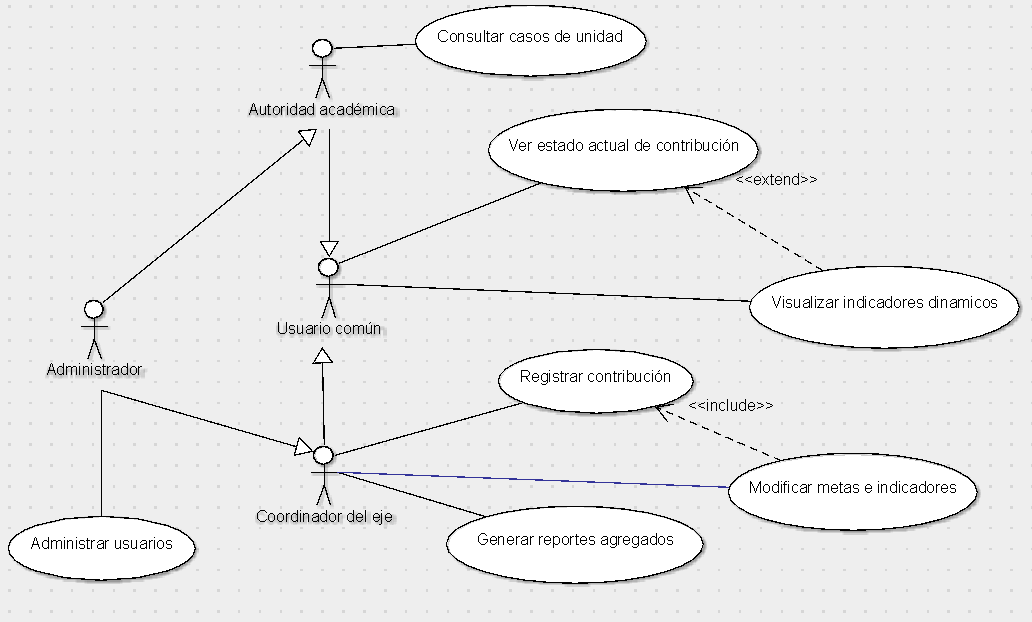
\includegraphics[width=0.8\textwidth]{image.png}
\end{center}

\subsubsection*{Actores}

\begin{enumerate}
  \item{\textbf{Administrador:} Permitir que los datos sean accesibles de forma segmentada según el nivel jerárquico dentro de la institución, desde autoridades de facultad hasta personal administrativo y académico.}
  \item{\textbf{Coordinador de Eje:} Responsable de uno de los tres ejes de acción (Formación Académica, Investigación, Vinculación con el Medio).}
  \item{\textbf{Autoridad Académica:} Puede ser el decano, director de departamento, etc., quien necesita ver el estado de contribución a los ODS de su unidad.}
  \item{\textbf{Usuario Común:} Cualquier empleado o miembro de la Universidad que necesita consultar el estado de una contribución.}   
\end{enumerate}
\subsubsection*{Casos de Uso}
\begin{enumerate}
  \item{\textbf{Registrar Contribución a ODS:} Permitir a los coordinadores de eje registrar o actualizar la contribución de diferentes ítemes a los ODS.}
  \item{\textbf{Ver estado actual de Contribución:} Mostrar el estado actual de la contribución, los ítemes específicos a los que aporta y quienes estén involucrados.}
  \item{\textbf{Generar Reportes Agregados:} Crear reportes que compilen los datos de contribución a los ODS.}
  \item{\textbf{Consultar Datos de Unidad:} Permitir a las autoridades académicas consultar los datos de su respectiva unidad.}
  \item{\textbf{Administrar Usuarios:} Añadir o eliminar usuarios y asignar sus roles.}
  \item{\textbf{Visualizar Indicadores Dinámicos:}  Ver gráficos  de estadísticas que muestran la evolución de la contribución a través del tiempo.}
  \item{\textbf{Modificar Metas e Indicadores:} Modificar los objetivos y condiciones de la contribución a medida que evoluciona.}
\end{enumerate}

\clearpage
\subsection{Documentación de Casos de Uso}

\begin{figure}[h]
  \centering
  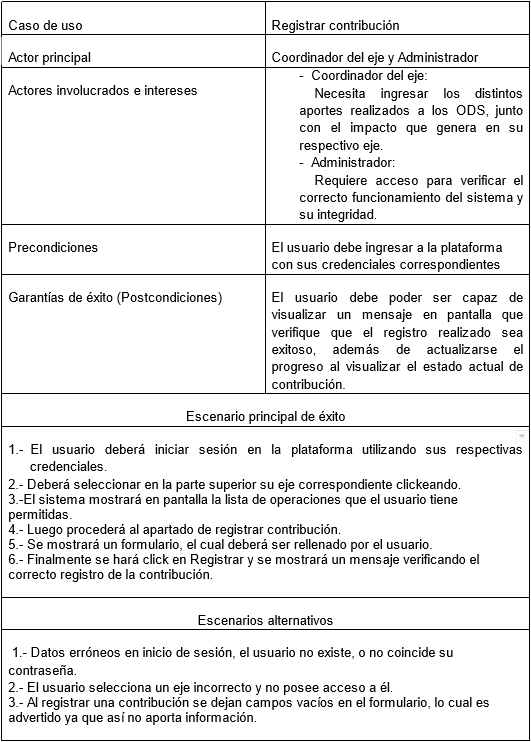
\includegraphics[width=0.75\textwidth]{caso1.png}
\end{figure}

\begin{figure}[h]
  \centering
  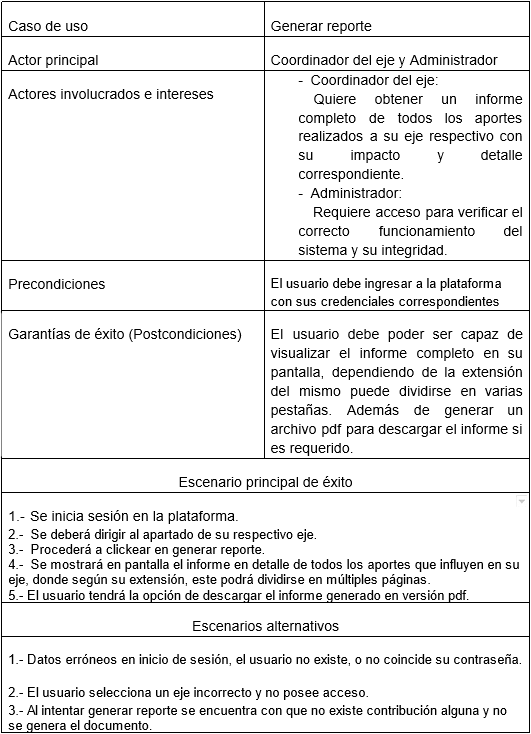
\includegraphics[width=0.75\textwidth]{caso2.png}
\end{figure}

\begin{figure}[h]
  \centering
  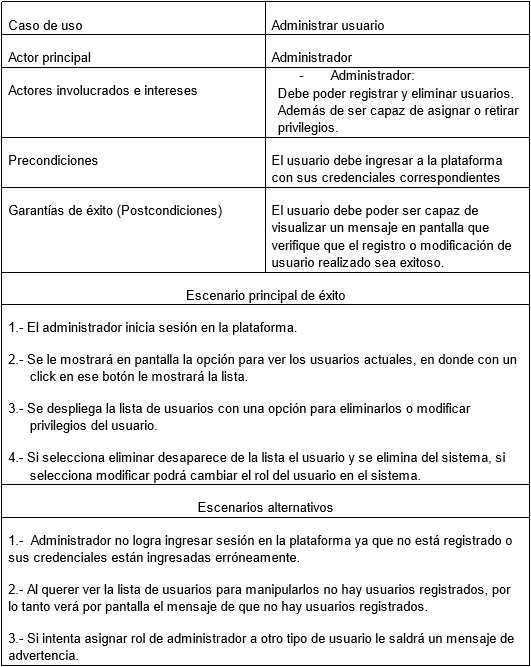
\includegraphics[width=0.75\textwidth]{caso3.png}
\end{figure}

\clearpage
\subsection{Esquema Conceptual}
\vspace{50pt}
\begin{figure}[h]
  \centering
  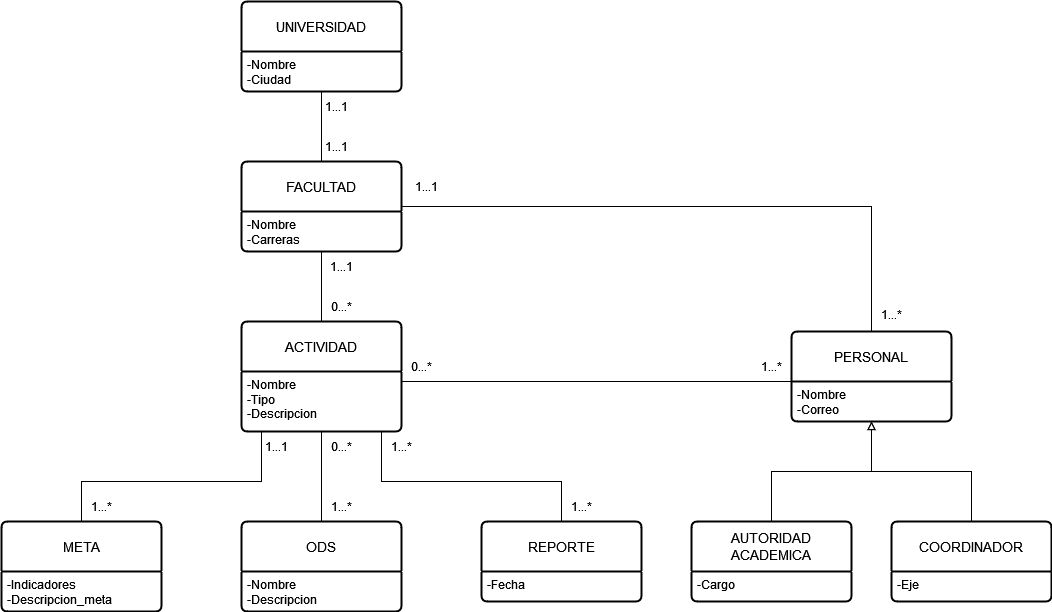
\includegraphics[width=1\textwidth]{esquema.png}
\end{figure}
\clearpage
\section{Conclusión}

La creación de un software para el monitoreo y contribución a los Objetivos de Desarrollo Sostenible (ODS) en la Universidad de Concepción se distingue por varios logros y desafíos. 

Uno de los desafíos más notables sería la centralización de todos los datos relacionados con los ODS. Esta característica es esencial, dado que antes de la implementación del software, la información se podría encontrar muy dispersa y de difícil acceso. Para superar este obstáculo, se optó por el uso de modelos de datos robustos y escalables que permitan una fusión efectiva de la información.

Junto con esto, el proyecto enfrentó dificultades en la creación de los indicadores dinámicos. El modelado de estos indicadores es un proceso bastante difícil que exige un análisis cuidadoso. Se optó por un modelo que permite la actualización y modificación de los indicadores sin requerir cambios importantes en el código, asegurando así la flexibilidad del sistema.

A pesar de las dificultades, un logro relevante fue la idea de implementar funciones para generar reportes y gráficos. Estas opciones no sólo cumplirían con la necesidad de los usuarios, como los docentes y estudiantes, sino que también son importantes para los administradores que supervisan la contribución a los ODS en la institución.

Otro logro a destacar sería la idea de implementar un sistema para que la información se pueda ver de forma inmediata y actualizada, permitiendo a las distintas autoridades y administrativos recibir información en tiempo real sobre la contribución de sus proyectos a los ODS.

Finalmente, se puede decir que el desarrollo del software se ha visto marcado por logros significativos en la generación de reportes y adaptabilidad del sistema, aunque también han presentado desafíos en términos de centralización de datos. En conclusión, este proyecto es una muy buena opción para que las instituciones educativas puedan contribuir de una manera mas eficiente a los Objetivos de Desarrollo Sostenible.




\end{document}